\subsection{Theory}

The entropy is calculated for all data points an order for the decisions must be found.
If a single decision can give information about a class or the removal of a class it is considered to be a high information gain.
Thus such a decision must be taken at the root of the tree.
But since the data provided to the tree cannot be 100\% of future all data to ever come, as it is with random input such as handwriting, every split carries a certain confidence.

\begin{figure}[h]
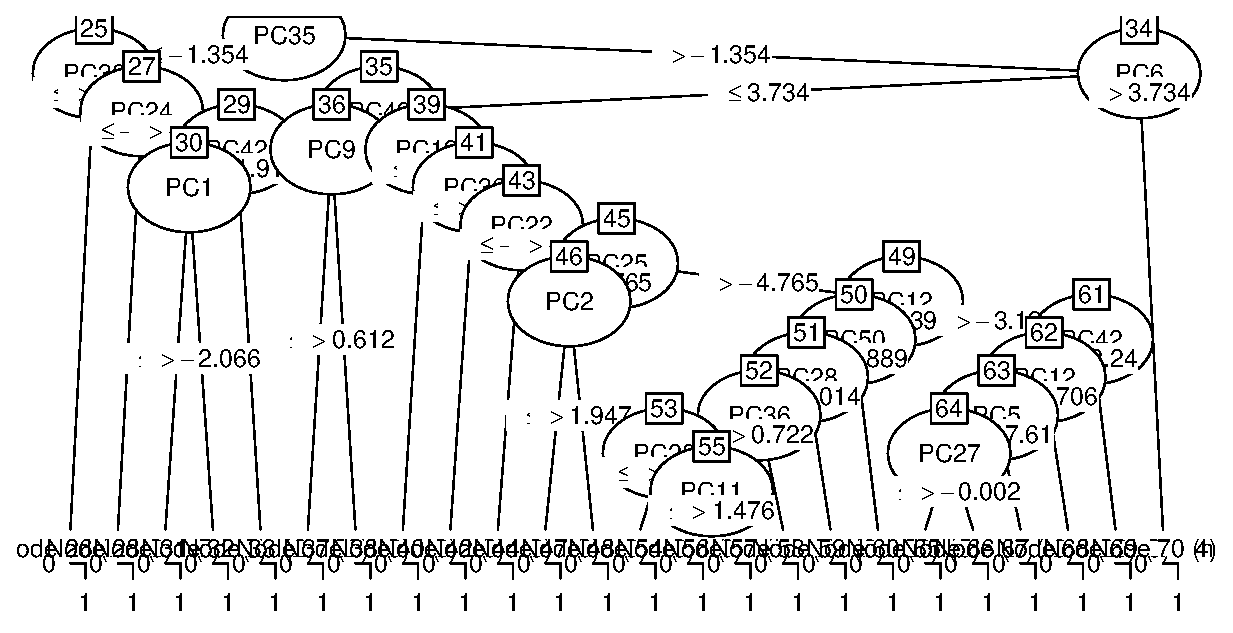
\includegraphics[width = \textwidth]{graphics/tree_section}
\caption[Visualization of a tree.]{Visualization of a small section of the tree.}
\label{fig:tree_section}
\end{figure}

Building a tree can be done using the ``C50'' library in R.
% The tree with the training data of 15 people (56000 cases) contains 6338 nodes.
A small section of the tree is shown in figure \ref{fig:tree_section}.
Each node shows which principal component and the split to which the decision is made.
Each leaf shows the probability of a classification.
The leftmost leaf (node 20) has n=2. This means that there are 2 cases where the decision splitting leads down to this node.
Both nodes are of class 10 so there is 100\% confidence that the number is of class 10.
On the right there is 65 cases in which the result is of class 1. 
This is a better indicator as it does not appear to be an random error in the data set.
The rightmost node has 4 results of the training data and cannot give a clear picture.
One is of class 4, one of 8 and two of class 10. 
When training this data half of the numbers will be misclassified.

A way to improve the decision tree is to remove nodes which is deemed to not be of significance.
This is called pruning, borrowing the vocabulary of gardening.
There are several ways to prune a tree.
The ``C5.0'' function can prune by increasing the confidence factor. 
The default is 25\% and thus a leaf with 1/4 confidence is allowed node 22 in figure \ref{fig:tree_section}.
If this number were increased the node would disappear.
This will lead to three sub nodes, differentiating the data.
Another pruning option is to increase the minimum number of nodes in a leaf. 
This will remove the noise created by a few selection of digits which creates a new split.
The default minimum number of nodes is 2.
Having this number too high will cause the confidence to go down as digits are lumped together. 